\documentclass{standalone}
\usepackage{tikz}
\usetikzlibrary{shapes.geometric, arrows.meta}

\tikzset{
    block/.style = {rectangle, draw=black, fill=white, text width=5em, text centered, rounded corners, minimum height=4em},
    arrow/.style = {thick,->,>=stealth}
}

\begin{document}
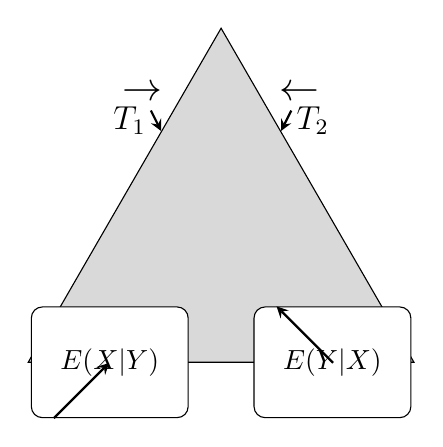
\begin{tikzpicture}[node distance=2cm]

    % Nodes
    \node (triangle) [draw=black, fill=gray!30, regular polygon, regular polygon sides=3, inner sep=1cm] {};
    
    \node (eq1) [block, below left of=triangle] {$E(X|Y)$};
    \node (eq2) [block, below right of=triangle] {$E(Y|X)$};
    
    \node (arrow1) [above of=triangle, xshift=-1cm] {\Large $\rightarrow$};
    \node (arrow2) [above of=triangle, xshift=1cm] {\Large $\leftarrow$};
    
    % Arrows
    \draw [arrow] (eq1) -- (triangle);
    \draw [arrow] (triangle) -- (eq2);
    \draw [arrow] (arrow1) -- node[anchor=east]{\large $T_1$} (triangle);
    \draw [arrow] (arrow2) -- node[anchor=west]{\large $T_2$} (triangle);

\end{tikzpicture}
\end{document}